\begin{frame}{Les types de bridges}
 Protocoles de communication et d'échanges entre différentes blockchains.
 Echange de données / d'actifs \newline \newline
 Plusieurs types de bridges :
 \begin{itemize}
     \item Trusted
     \item Trustless
 \end{itemize} 
 Différentes manières d'échanger les actifs:
 \begin{itemize}
     \item Lock and Mint
     \item Burnt and Mint
     \item Atomic Swaps
 \end{itemize}
\end{frame}

\begin{frame}{Trusted Blockchain Bridge}
    Basés sur une entité centrale en tant que tiers de confiance.
Des informations clés: 
    \begin{itemize}
        \item Façilite les transferts.
        \item Utilisation simple.
        \item Échanges sécurisés.
        \item Possible remboursement en cas de cyberattaque.
        \item Cible façile.
    \end{itemize}
    $\Rightarrow$ MAIS l'utilisateur donne le contrôle de ses actifs.\\ 
Exemple de Trusted Bridge : Binance Bridge.
\end{frame}

\begin{frame}{Trustless Blockchain Bridge}
Basés sur un réseau décentralisé 
Des informations clés: 
\begin{itemize}
    \item Aucune présence d'un tiers de confiance.
    \item Sécurité du bridge égale à celle de la chaîne sous-jacente.
    \item Permettent aux utilisateurs de contrôler leurs actifs.
    \item Aucune garantie en cas de hack.
\end{itemize}
Exemple de trustless bridge : Polygon Bridge.
\end{frame}

\begin{frame}{Mécanisme de vérification}
Les mécanismes de vérification des bridges peuvent être classés en trois types:
\begin{itemize}
    \item Locale (ex: Hop/Connext legacy)
    \item Extérieure (ex: Avalanche Bridge)
    \item Native (ex: The NEAR Rainbow Bridge)
\end{itemize}
\end{frame}


\begin{frame}{Vérification locale, native et externe}
    \begin{figure}
        \centering
        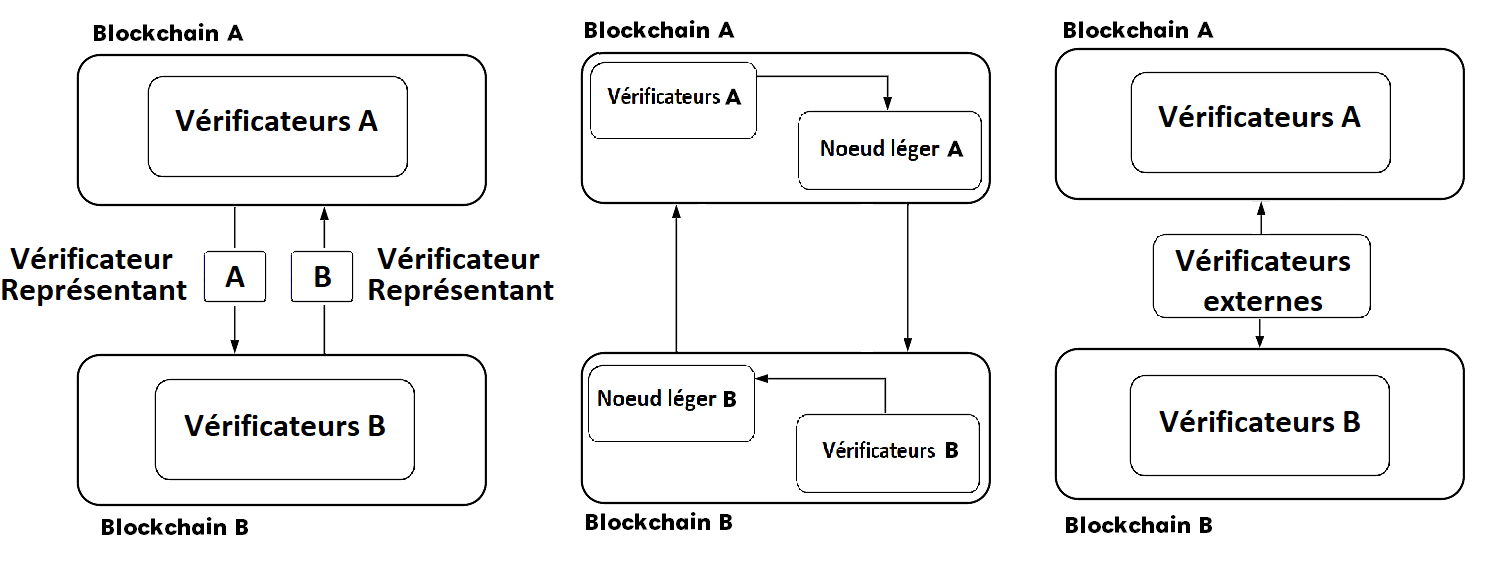
\includegraphics[scale = 0.5]{img/DiagrammeResumeVerif.png}
    \end{figure}
\end{frame}

\begin{frame}{Le trilemme de l’interopérabilité}
    Repose sur 3 notions: 
    \begin{figure}
        \centering
        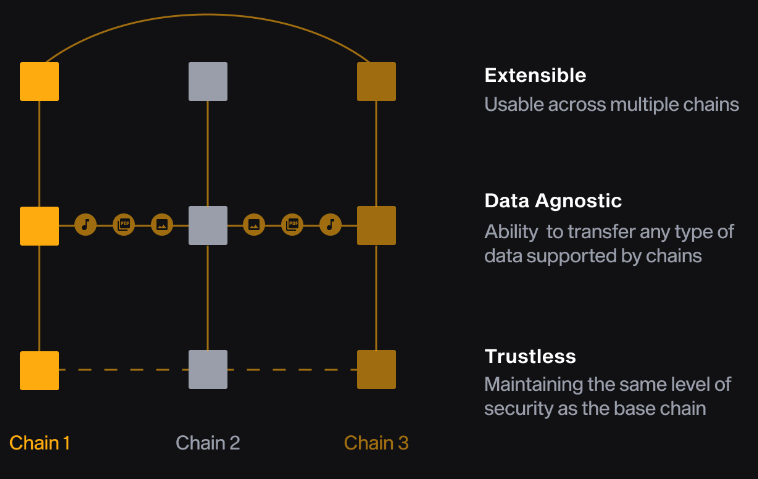
\includegraphics[scale = 0.7]{img/3notions.png}
    \end{figure}
    \end{frame}

\begin{frame}{Solution optimiste}
Bridge optimiste avec de l'importance sur la sécurité plutôt que sur la vivacité.
Déroulement : \newline
\begin{itemize}
    \item Envoi de données vers une fonction contrat.
    \item Validation de la transaction par un vérificateur. 
    \item Ajout d'un collatéral de la part du vérificateur. 
    \item Envoi sur une chaîne destination par un \textit{relayer}. 
    \item 30 minutes de latence pour prouver une fraude.
    \item Les données sont passées à la chaîne destination puis traitées.
\end{itemize}
\end{frame}

\begin{frame}{Possibles faiblesses et leurs solutions}
\begin{itemize}
    \item \textit{Updater DoS}
        \begin{itemize}
            \item Mécanisme de substitution.
            \item Perte du collatéral.
        \end{itemize}
    \item \textit{Updater Fraud} \begin{itemize} \item Perte du collatéral. \end{itemize}
    \item \textit{Watcher DoS} 
        \begin{itemize}
            \item Signalement de fraude payant.
            \item Perte du collatéral.
            \item Vérificateurs approuvés.
        \end{itemize}
\end{itemize}
\end{frame}

\begin{frame}{Les faiblesses des bridges}
\begin{itemize}
    \item \textit{Trustless Bridges} : Les \textit{smart contracts} et l'erreur humaine.
    \item \textit{Trusted Bridges} : Les fraudes \textit{rug pull}.
    \item Une technologie récente.
    \item L'\textit{open source}.
\end{itemize}
\end{frame}
